\section{Field Probing Neural Network}
\label{sec:fpnn}

%\vspace{-0.2cm}

\subsection{Input 3D Fields}
\label{sec:input_3d_fields}

\begin{wrapfigure}{R}{0.5\linewidth}
	\vspace{-2.9cm}
	\begin{center}
		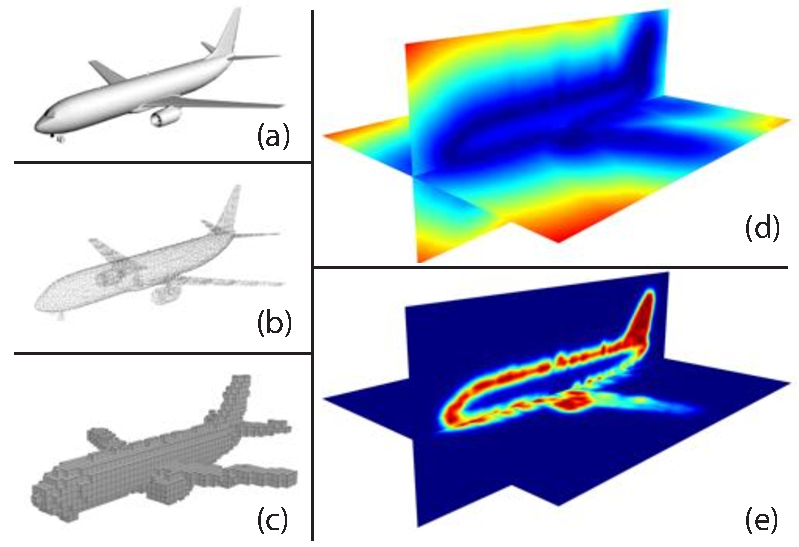
\includegraphics[width=0.9\linewidth]{figures/3d_data_representations}
	\end{center}
	\vspace{-0.5cm}
	\caption{3D mesh (a) or point cloud (b) can be converted into occupancy grid (c), from which the input to our algorithm --- a 3D distance field (d), is obtained via a distance transform. We further transform it to a Gaussian distance field (e) for focusing attention to the space near the surface. The fields are visualized by two crossing slices.}
	\label{fig:3d_data_representations}
	\vspace{-0.4cm}
\end{wrapfigure}

We study the 3D shape classification problem by employing a deep neural network. The input of our network is a 3D vector field built from the input shape and the output is an object category label. 3D shapes represented as meshes or point clouds can be converted into 3D distance fields. Given a mesh (or point cloud), we first convert it into a binary occupancy grid representation, where the binary occupancy value in each grid is determined by whether it intersects with any mesh surface (or contains any sample point). Then we treat the occupied cells as the zero level set of a surface, and apply a distance transform to build a 3D distance field $\mathcal{D}$, which is stored in a 3D array indexed by $(i,j,k)$, where $i,j,k = 1,2,...,R$, and $R$ is the resolution of the distance field. We denote the distance value at $(i,j,k)$ by $\mathcal{D}_{(i,j,k)}$. Note that $\mathcal{D}$ represents distance values at discrete grid locations. The distance value at an arbitrary location $d(x,y,z)$ can be computed by standard trilinear interpolation over $\mathcal{D}$. See Figure~\ref{fig:3d_data_representations} for an illustration of the 3D data representations.

Similar to 3D distance fields, other 3D fields, such as normal fields $\mathcal{N}_x$, $\mathcal{N}_y$, and $\mathcal{N}_z$, can also be used for representing shapes.
Note that the normal fields can be derived from the gradient of the distance field:
%\begin{equation}
$
{\mathcal{N}_x}(x,y,z) = \frac{1}{l}\frac{\partial d}{\partial x},
{\mathcal{N}_y}(x,y,z) = \frac{1}{l}\frac{\partial d}{\partial y},
{\mathcal{N}_z}(x,y,z) = \frac{1}{l}\frac{\partial d}{\partial z},
$
%\label{eq:normal_fields}
%\end{equation}
where $l=|(\frac{\partial d}{\partial x}, \frac{\partial d}{\partial y}, \frac{\partial d}{\partial z})|$.
% Note that the gradient in these normal fields can be evaluated by Equation~\ref{eq:3d_field_gradients} in these fields themselves, which are actually the second order derivatives of the distance field.
Our framework can employ any set of fields as input, as long as the gradients can be computed.

\subsection{Field Probing Layers}
\label{sec:fpnn_layers}

\begin{wrapfigure}{R}{0.5\linewidth}
	\vspace{-1.8cm}
	\begin{center}
		\includegraphics[width=0.9\linewidth]{figures/initialization}
	\end{center}
	\vspace{-0.4cm}
	\caption{Initialization of field probing layers. For simplicity, a subset of the filters are visualized.}
	\label{fig:initialization}
	\vspace{-0.3cm}
\end{wrapfigure}

The basic modules of deep neural networks are layers, which gradually convert input to output in a \emph{forward pass}, and get updated during a \emph{backward pass} through the \emph{Back-propagation}~\cite{Williams_Nature86_Learning} mechanism.
%
%The basic modules of deep neural networks are layers. Each layer is a simple function $f$ together with its parameters $W$, taking an input $X$ and mapping it into another representation $Y = f(X, W)$. The procedure that maps input $X$ into output $Y$ is called a \emph{forward pass}. The inverse of the forward pass, \emph{backward pass}, computes the gradient $\nabla f$ for updating $X$ and $W$ to optimize $Y$. \emph{Back-propagation}~\cite{Williams_Nature86_Learning} recursively applies \emph{chain rule} to propagate gradients all the way back into the layers that build up the network and get the layer parameters updated. Being able to compute the gradients $\nabla f$ in the layers is the key for making the composite network trainable so as to learn features from input data.
%
The key contribution of our approach is that we replace the convolutional layers in CNNs by field probing layers, a novel component that uses field probing filters to efficiently extract features from the 3D vector field. They are composed of three layers: \emph{Sensor layer}, \emph{DotProduct layer} and \emph{Gaussian layer}. The Sensor layer is responsible for collecting the signals (the values in the input fields) at the probing points in the forward pass, and updating the probing point locations in the backward pass. The DotProduct layer computes the dot product between the probing filter weights and the signals from the Sensor layer. The Gaussian layer is an utility layer that transforms distance field into a representation that is more friendly for numerical computation. We introduce them in the following paragraphs, and show that they fit well for training a deep network.

\paragraph{Sensor Layer.} The input to this layer is a 3D field $\mathcal{V}$, where $\mathcal{V}(x,y,z)$ yields a $T$ channel ($T=1$ for distance field and $T=3$ for normal fields) vector at location $(x,y,z)$. This layer contains $C$ probing filters scattered in space, each with $N$ probing points. The parameters of this layer are the locations of all probing points $\{(x_{c,n},y_{c,n},z_{c,n})\}$, where $c$ indexes the filter and $n$ indexes the probing point within each filter. This layer simply outputs the vector at the probing points $\mathcal{V}(x_{c,n},y_{c,n},z_{c,n})$. The output of this layer forms a data chunk of size $C \times N \times T$.

The gradient of this function $\nabla \mathcal{V} =(\frac{\partial \mathcal{V}}{\partial x}, \frac{\partial p}{\partial y}, \frac{\partial p}{\partial z})$ can be evaluated by numerical computation, which will be used for updating the locations of probing points in the back-propagation process. This formal definition emphasizes why we need the input being represented as 3D fields: the gradients computed from the input fields are the forces to push the probing points towards more informative locations until they converge to a local optimum.

\paragraph{DotProduct Layer.} The input to this layer is the output of the Sensor layer --- a data chunk of size $C \times N \times T$, denoted as $\{p_{c,n,t}\}$. The parameters of DotProduct layer are the filter weights associated with probing points, i.e., there are $C$ filters, each of length $N$, in $T$ channels. We denote the set of parameters as $\{w_{c,n,t}\}$. The function at this layer computes a dot product between $\{p_{c,n,t}\}$ and $\{w_{c,n,t}\}$, and outputs
$
%\begin{equation}
v_{c} = v(\{p_{c,i,j}\}, \{w_{c,i,j}\}) = \sum_{\substack{
   i=1,...,N \\
   j=1,...,T
  }} p_{c,i,j} \times w_{c,i,j},
%\end{equation}
$
--- a $C$-dimensional vector, and the gradient for the backward pass is:
$
%\begin{equation}
\nabla v_c =(\frac{\partial v}{\partial \{p_{c,i,j}\}}, \frac{\partial v}{\partial \{w_{c,i,j}\}}) = (\{w_{c,i,j}\}, \{p_{c,i,j}\}).
%\end{equation}
$

Typical convolution encourages weight sharing within an image patch by ``zipping'' the patch into a single value for upper layers by a dot production between the patch and a 2D filter. Our DotProduct layer shares the same ``zipping'' idea, which facilitates to fully connect it: probing points are grouped into probing filters to generate output with lower dimensionality. 

Another option in designing convolutional layers is to decide whether their weights should be shared across different spatial locations. In 2D CNNs, these parameters are usually shared when processing general images. In our case, we opt not to share the weights, as information is not evenly distributed in 3D space, and we encourage our probing filters to individually deviate for adapting to the data.

\paragraph{Gaussian Layer.} Samples in locations distant to the object surface are associated with large distance values from the distance field. Directly feeding them into the DotProduct layer does not converge and thus does not yield reasonable performance. To emphasize the importance of samples in the vicinity of the object surface, we apply a Gaussian transform (inverse exponential) on the distances so that regions approaching the zero surface have larger weights while distant regions matter less.\footnote{Applying a batch normalization~\cite{ioffe2015batch} on the distances also resolves the problem. However, Gaussian transform has two advantages: 1. it can be approximated by truncated distance fields~\cite{Curless_SIGGRAPH96_A}, which is widely used in real time scanning and can be compactly stored by voxel hashing~\cite{Niessner_ToG13_Real}, 2. it is more efficient to compute than batch normalization, since it is element-wise operation.}. We implement this transform with a Gaussian layer. The input is the output values of the Sensor layer. Let us assume the values are $\{x\}$, then this layer applies an element-wise Gaussian transform $g(x) = e^{-\frac{x^2}{2 {\sigma}^2}}$, and the gradient is $\nabla g = -\frac{x e^{-\frac{x^2}{2 {\sigma}^2}}}{{\sigma}^2}$ for the backward pass.

%Mathematically, we can switch the order of the Sensor layer and Gaussian layer, i.e., we can first transform the distance field by the Gaussian layer and then sample the locations. However, since we numerically compute $\nabla d$ by tri-linear interpolation of values at discrete grid locations, and the Gaussian transform would increase the non-linearity of the input fields, applying the Sensor layer first yields better numerical stability.

%The Gaussian transform can be viewed as a soft version of the truncation operation in truncated distance fields~\cite{Curless_SIGGRAPH96_A}, a representation widely used in real time scanning and reconstruction. Therefore, our system can easily be integrated into existing scanning and reconstruction frameworks. Furthermore, the input distance field can be compactly stored by voxel hashing~\cite{Niessner_ToG13_Real} to reduce the I/O footprint.

\paragraph{Complexity of Field Probing Layers.} The complexity of field probing layers is $O(C \times N \times T)$, where $C$ is the number of probing filters, $N$ is the number of probing points on each filter, and $T$ is the number of input fields. The complexity of the convolutional layer is $O(K^3 \times C \times S^3)$, where $K$ is the 3D kernel size, $C$ is the output channel number, and $S$ is the number of the sliding locations for each dimension. In field probing layers, we typically use $C = 1024$, $N = 8$, and $T=4$ (distance and normal fields), while in 3D CNN $K=6$, $C = 48$ and $S=12$. Compared with convolutional layers, field probing layers save a majority of computation ($1024 \times 8 \times 4 \approx 1.83\% \times 6^3 \times 48 \times 12^3$), as the probing filters in field probing layers are capable of learning where to ``sense'', whereas convolutional layers exhaustively examine everywhere by sliding the 3D kernels.

\paragraph{Initialization of Field Probing Layers.}

There are two sets of parameters: the probing point locations and the weights associated with them. To encourage the probing points to explore as many potential locations as possible, we initialize them to be widely distributed in the input fields. We first divide the space into $G \times G \times G$ grids and then generate $P$ filters in each grid. Each filter is initialized as a line segment with a random orientation, a random length in $[l_{low}, l_{high}]$ (we use $[l_{low}, l_{high}]=[0.2, 0.8]*R$ by default), and a random center point within the grid it belongs to (Figure~\ref{fig:initialization} left). Note that a probing filter spans distantly in the 3D space, so they capture long range effects well. This is a property that distinguishes our design from those convolutional layers, as they have to increase the kernel size to capture long range effects, at the cost of increased complexity. The weights of field probing filters are initialized by the Xavier scheme~\cite{glorot2010understanding}. In Figure~\ref{fig:initialization} right, weights for distance field are visualized by probing point colors and weights for normal fields by arrows attached to each probing point.
%An interpretation to weights for normal fields is that they are vectors that parametrize directional lights, whose energies are the magnitudes of the vector and the directions are the orientation of the vector. Under this interpretation, the inner product between the weight vector and normal fields corresponds to the perceived intensity at probing points. Additionally, our learning scheme optimizes the light parameters for collecting more informative responses.

\begin{wrapfigure}{R}{0.45\linewidth}
	\vspace{-1.4cm}
	\begin{center}
		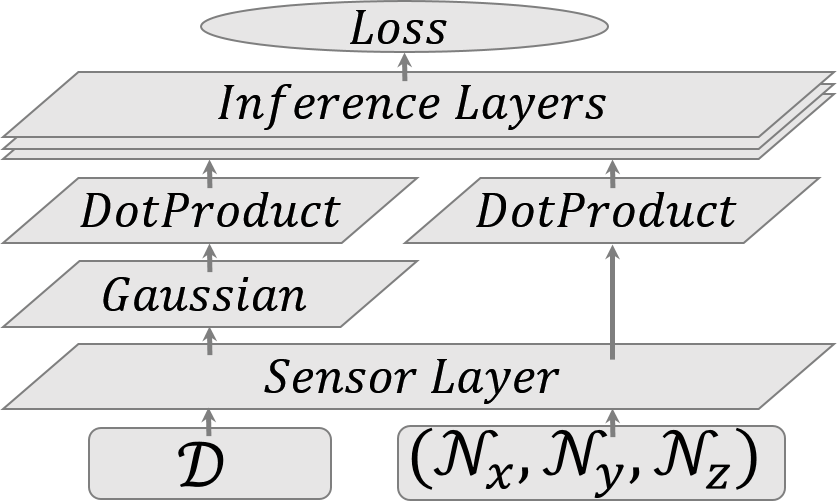
\includegraphics[width=1.0\linewidth]{figures/fpnn_architecture}
	\end{center}
	\vspace{-0.4cm}
	\caption{FPNN architecture. Field probing layers can be used together with other inference layers to minimize task specific losses.}
	\label{fig:fpnn_architecture}
	\vspace{-0.5cm}
\end{wrapfigure}

\paragraph{FPNN Architecture and Usage.} Field probing layers transform input 3D fields into an intermediate representation, which can further be processed and eventually linked to task specific loss layers (Figure~\ref{fig:fpnn_architecture}). To further encourage long range connections, we feed the output of our field probing layers into fully connected layers. The advantage of long range connections makes it possible to stick with a small number of probing filters, while the small number of probing filters makes it possible to directly use fully connected layers.

Object classification is widely used in computer vision as a testbed for evaluating neural network designs, and the neural network parameters learned from this task may be transferred to other high-level understanding tasks such as object retrieval and scene parsing. Thus we choose 3D object classification as the task for evaluating our FPNN.

